% Overview of the study (Figure 1). Drawn in TikZ so that it uses the paper's fonts; \input by sections/method.tex.
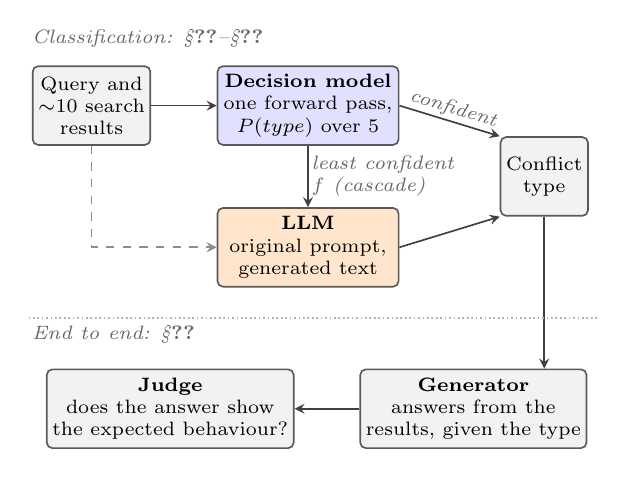
\begin{tikzpicture}[
  font=\scriptsize, >=stealth, line width=0.6pt,
  box/.style={draw=black!65, rounded corners=2pt, align=center, inner sep=2pt, minimum height=10mm},
  note/.style={font=\scriptsize\itshape, text=black!60, align=center, inner sep=1pt},
  arr/.style={->, draw=black!75}]
  % Classification.
  \node[box, fill=black!5, minimum width=14mm] (in) at (0, 0) {Query and\\$\sim$10 search\\results};
  \node[box, fill=blue!12, minimum width=23mm] (dm) at (2.75, 0) {\textbf{Decision model}\\one forward pass,\\$P(\text{type})$ over 5};
  \node[box, fill=orange!20, minimum width=23mm] (llm) at (2.75, -1.8) {\textbf{LLM}\\original prompt,\\generated text};
  \node[box, fill=black!5, minimum width=11mm] (type) at (5.75, -0.9) {Conflict\\type};
  \draw[arr] (in) -- (dm);
  \draw[arr] (dm.east) -- node[note, above, sloped] {confident} (type.north west);
  \draw[arr] (dm.south) -- node[note, right, align=left] {least confident\\$f$ (cascade)} (llm.north);
  \draw[arr] (llm.east) -- (type.south west);
  \draw[arr, dashed, draw=black!45] (in.south) |- (llm.west);
  % End to end.
  \node[box, fill=black!5, minimum width=27mm] (gen) at (4.85, -3.85) {\textbf{Generator}\\answers from the\\results, given the type};
  \node[box, fill=black!5, minimum width=27mm] (judge) at (1.0, -3.85) {\textbf{Judge}\\does the answer show\\the expected behaviour?};
  \draw[arr] (type.south) -- (type.south |- gen.north);
  \draw[arr] (gen) -- (judge);
  % Where each part is evaluated.
  \draw[black!30, densely dotted] (-0.8, -2.7) -- (6.45, -2.7);
  \node[note, anchor=north west] at (-0.8, 1.0) {Classification: \S\ref{sec:main}--\S\ref{sec:diagnostics}};
  \node[note, anchor=north west] at (-0.8, -2.75) {End to end: \S\ref{sec:endtoend}};
\end{tikzpicture}
